\documentclass[a4paper,11pt]{article}

\usepackage[utf8]{inputenc}
\usepackage[T1]{fontenc}
\usepackage[margin=2.5cm]{geometry}
\usepackage{amsmath}
\usepackage{xcolor}
\usepackage{hyperref}
\usepackage{graphicx}


% code block style
\usepackage{listings}

\definecolor{codegreen}{rgb}{0,0.6,0}
\definecolor{codegray}{rgb}{0.5,0.5,0.5}
\definecolor{codepurple}{rgb}{0.58,0,0.82}
\definecolor{backcolour}{rgb}{0.95,0.95,0.92}

\lstdefinestyle{mystyle}{
    backgroundcolor=\color{backcolour},
    commentstyle=\color{codegreen},
    keywordstyle=\color{magenta},
    numberstyle=\tiny\color{codegray},
    stringstyle=\color{codepurple},
    basicstyle=\ttfamily\footnotesize,
    breakatwhitespace=false,
    breaklines=true,
    captionpos=b,
    keepspaces=true,
    numbers=left,
    numbersep=5pt,
    showspaces=false,
    showstringspaces=false,
    showtabs=false,
    tabsize=2
}
\lstset{style=mystyle}

% Settings
\usepackage[sc]{titlesec}
\newcommand{\comment}[1]{\noindent \textcolor{blue}{\textit{#1}} \par}

% Header information
\title{\Large{\sc{Performance Engineering}}\\[2mm] Lab 5}
\author{Jort Oosterveld S5545781 \& Sergiu Preda S6778542 \\ Group 11}

\begin{document}
\setlength\parindent{0pt}
\setlength{\parskip}{0.6em}

\maketitle

% ================================================================================
% Excercise 1
% ================================================================================
\section{Information Exchange analysis of a cache-blocked matrix-vector multiply}

The implementation of the cache-blocked matrix-vector multiplication can be seen in listing \ref{lst:matvec_cb}.
\begin{lstlisting}[ caption={Matrix-vector multiplication: cache-blocked implementation.}, label=lst:matvec_cb]
/* 
 * y = A * x using cache blocking
 * N: Matrix dimension (N x N)
 * B: Block size (N % B = 0)
 * A: Flattened N x N matrix 
 * x: Input vector of size N
 * y: Output vector of size N
 */
void blocked_mat_vec(int N, int B, const double *A, const double *x, double *y) {
    // 1. Initialize output vector
    for (int i = 0; i < N; i++) {
        y[i] = 0.0;
    }

    // 2. Iterate over blocks
    for (int i = 0; i < N; i += B) {          // Row blocks
        for (int j = 0; j < N; j += B) {      // Column blocks
            
            // 3. Compute multiplication for the current B x B block
            for (int ii = i; ii < i + B; ii++) {
                for (int jj = j; jj < j + B; jj++) {
                    y[ii] += A[ii * N + jj] * x[jj];
                }
            }
            
        }
    }
}
\end{lstlisting}

To calculate $I_{mem}$ for a matrix-vector multiplication of the form $\vec{y} = A \cdot \vec{x}$, we assume:
\begin{itemize}
    \item The entire vector $\vec{x}$ cannot be kept in cache.
    \item A fraction $N/B$ of the vector can stay in cache.
    \item The block size $B$ satisfies $N\%B = 0$.
\end{itemize}

This means there is still one load for every element of $A$, thus $8N^2$ bytes.
There is one load for every element in each block, thus $8\cdot(B\cdot N/B) = 8N$.
There is one load, and one store for every partial sum of the row (each block), thus $2 \cdot 8 \cdot N\cdot N/B = 16 \cdot N^2/B$.
The total number of stores and loads then adds up to:
\[
    I_{mem} = 8N^2 + 16N^2/B + 8N
\]

% ================================================================================
% Excercise 2
% ================================================================================
\section{Cachegrind}

The cache-blocked routine of Listing~\ref{lst:matvec_cb} was run under Cachegrind
(\texttt{valgrind --tool=cachegrind}) on Sergiu's machine (see
Section~\ref{section:hardware_info}), which has a 48~KiB L1D cache per core.
We selected $N = 8192$: with double-precision numbers (8 bytes per element) a
single vector of size $N$ occupies $8192 \times 8 = 65{,}536$ bytes (64~KiB),
which strictly exceeds the L1D cache capacity.

The bash script in Listing~\ref{lst:bash_script_matvec} executes the program for
the block sizes $B = 8, 16, 32, \ldots, 1024$ while keeping $N = 8192$ constant and extracts the \texttt{D1 misses} (L1 data cache misses)
from Cachegrind's output.

\begin{lstlisting}[language=Bash, caption={Script running the blocked matrix-vector multiply under Cachegrind for a range of block sizes.}, label=lst:bash_script_matvec]
#!/bin/bash

# Fixed matrix size (N=8192 ensures the vector exceeds the 48 KiB L1d cache)
N=8192

# Array of block sizes to test
BLOCK_SIZES=(8 16 32 64 128 256 512 1024)

# Output CSV file
OUTPUT_FILE="cache_misses.csv"

# Initialize the CSV with headers
echo "BlockSize_B,D1_Misses" > "$OUTPUT_FILE"
echo "Starting Cachegrind benchmark for N=$N..."

for B in "${BLOCK_SIZES[@]}"; do
    echo -n "Testing B=$B... "

    # --cachegrind-out-file=/dev/null prevents the .out files from being generated
    # awk '{print $4}' grabs the actual number instead of the word "misses:"
    MISSES=$(valgrind --tool=cachegrind --cachegrind-out-file=/dev/null ./blocked_matvec $N $B 2>&1 | grep "D1  misses:" | awk '{print $4}' | tr -d ',')

    # Append the result to the CSV
    echo "$B,$MISSES" >> "$OUTPUT_FILE"
    echo "Misses: $MISSES"
done

echo "Done! Results saved to $OUTPUT_FILE."
\end{lstlisting}

The results are listed in Table~\ref{tab:cache_misses} and visualized in
Figure~\ref{fig:cache_misses}.

\begin{table}[h]
    \centering
    \begin{tabular}{c c}
        Block size $B$ & D1 cache misses \\
        \hline
         8   & 17839350 \\
        16   & 21525718 \\
        32   & 19170454 \\
        64   & 17992726 \\
        128  & 17403671 \\
        256  & 17108263 \\
        512  & 16945895 \\
        1024 & 16863598 \\
        \hline
    \end{tabular}
    \caption{L1D cache misses for different block sizes with $N=8192$ (large enough that the vector does not fit in L1D), measured on Sergiu's system, see Section~\ref{section:hardware_info}.}
    \label{tab:cache_misses}
\end{table}

\begin{figure}[h]
    \centering
    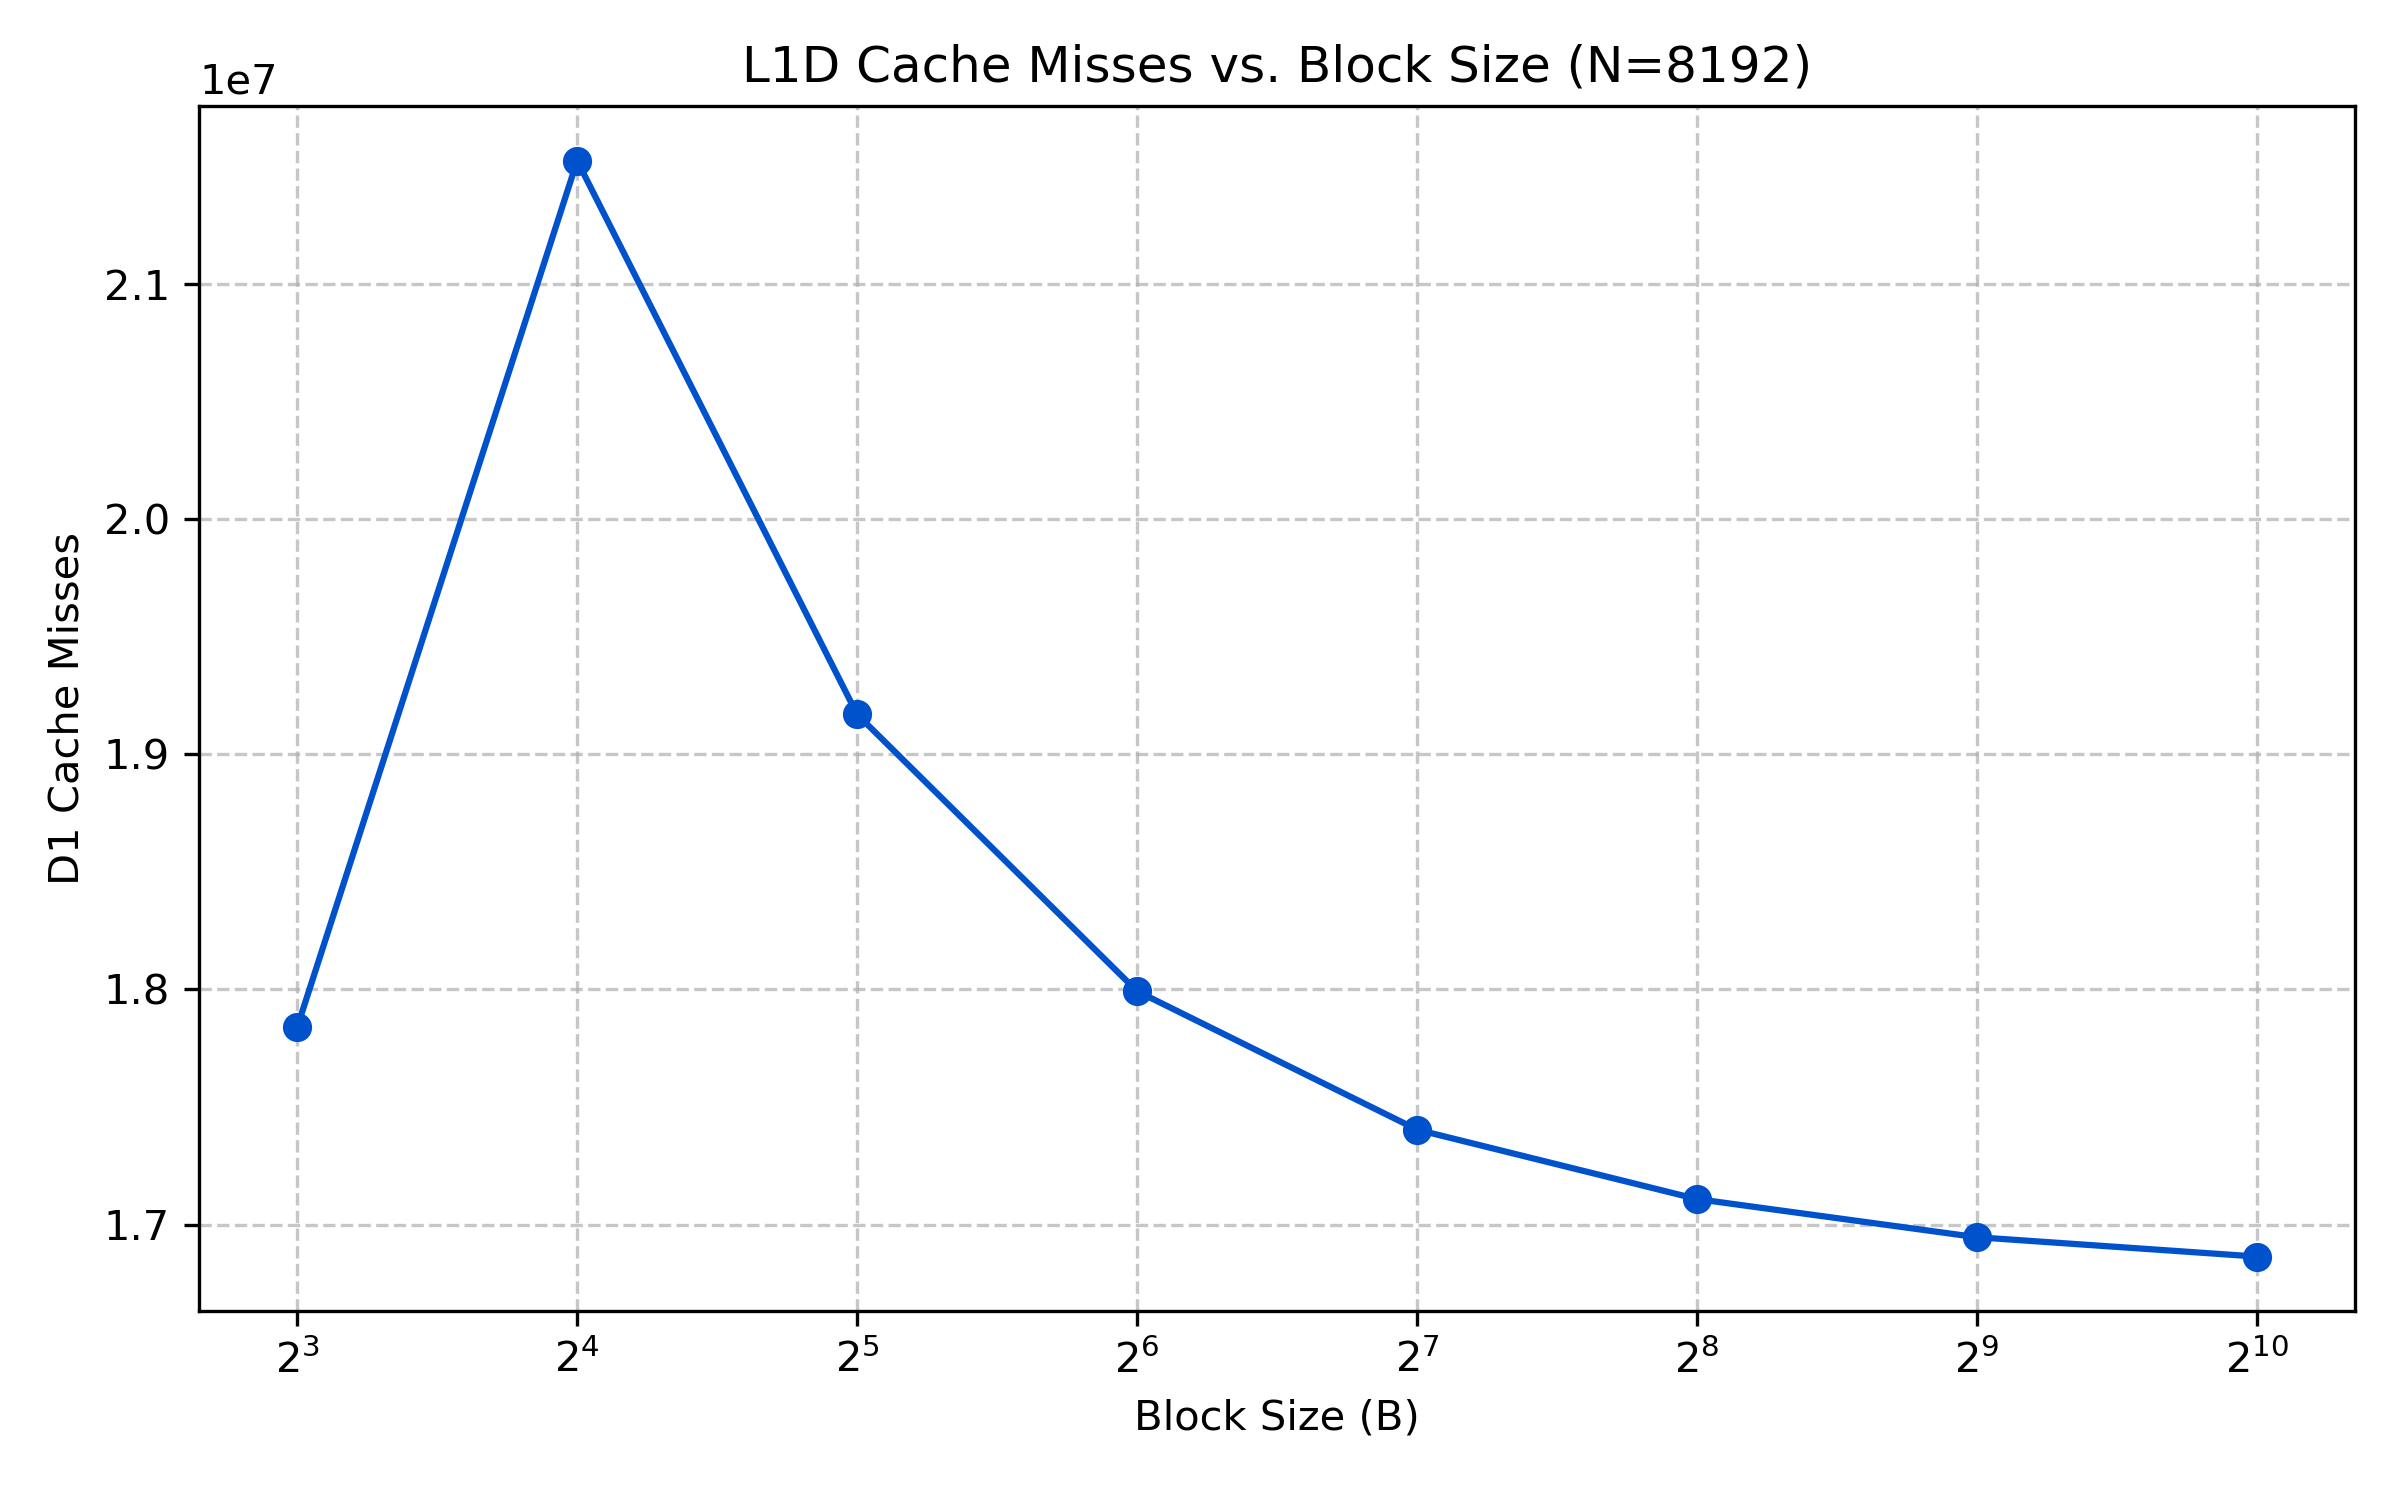
\includegraphics[width=0.7\textwidth]{figure_1_cache_misses.png}
    \caption{L1D cache misses as a function of block size $B$ for $N=8192$.}
    \label{fig:cache_misses}
\end{figure}

The graph shows that the number of cache misses peaks at small block sizes
(e.g., $B=16$) and drops significantly as the block size increases up to
$B=1024$. This indicates better utilization of the L1D cache capacity before
eviction becomes strictly necessary.

% ================================================================================
% Excercise 3
% ================================================================================
\section{Memory allocation overhead}

To measure the overhead of allocating and freeing memory dynamically we wrote
the C++ benchmark of Listing~\ref{lst:c_benchmark}. It uses
\texttt{clock\_gettime(CLOCK\_MONOTONIC)} to measure the time of a malloc and free pair for different sizes.
It does this in two ways, for consistency:

\begin{enumerate}
    \item \textbf{Batch timing:} the timer is read once, $1e6$
    malloc/free pairs are executed, the timer is read again
    and the elapsed time is divided by the number of pairs.
    \item \textbf{Per-pair timing:} every single pair is wrapped in two timer
    reads, so that the full distribution (mean, median, standard deviation,
    minimum, maximum) of $1e6$ samples is obtained. The cost of the timer
    itself is measured separately and subtracted.
\end{enumerate}

The allocated block is touched with a \texttt{volatile} store before it is
freed, because otherwise the compiler can remove the dead code.
Every size is preceded by an unmeasured warm-up pass of $10^5$ pairs to remove any one-time costs.

\begin{lstlisting}[language=C++, caption={Benchmark for the overhead of a \texttt{malloc}/\texttt{free} pair (\texttt{benchmark\_malloc.cpp}, statistics bookkeeping omitted).}, label=lst:c_benchmark]
static const clockid_t CLOCK_ID = CLOCK_MONOTONIC;

static inline long long timespec_diff_ns(const struct timespec *t2,
                                         const struct timespec *t1)
{
    return ((long long)(t2->tv_sec - t1->tv_sec) * 1000000000LL) +
           (t2->tv_nsec - t1->tv_nsec);
}

/* running mean / variance, min, max and median
 * of all samples added with add(). */
struct TimingStats { /* ... */ void add(long long ns); double mean; /* ... */ };

/* Cost of two back-to-back clock_gettime() calls */
static TimingStats measure_timer_overhead(int iterations)
{
    TimingStats stats;
    struct timespec t1, t2;
    for (int i = 0; i < iterations; ++i) {
        clock_gettime(CLOCK_ID, &t1);
        clock_gettime(CLOCK_ID, &t2);
        stats.add(timespec_diff_ns(&t2, &t1));
    }
    return stats;
}

/* individual pair timing */
static TimingStats measure_alloc_per_pair(size_t alloc_size, int iterations)
{
    TimingStats stats;
    struct timespec start, end;
    for (int i = 0; i < iterations; i++) {
        clock_gettime(CLOCK_ID, &start);
        void *ptr = malloc(alloc_size);
        // touch the memory so the allocation cannot be optimised away
        if (ptr != NULL) {
            ((volatile char *)ptr)[0] = 'a';
            free(ptr);
        }
        clock_gettime(CLOCK_ID, &end);
        stats.add(timespec_diff_ns(&end, &start));
    }
    return stats;
}

/* batch timing, clock overhead is insignificant */
static double measure_alloc_batch(size_t alloc_size, int iterations)
{
    struct timespec start, end;
    clock_gettime(CLOCK_ID, &start);
    for (int i = 0; i < iterations; i++) {
        void *ptr = malloc(alloc_size);
        if (ptr != NULL) {
            ((volatile char *)ptr)[0] = 'a';
            free(ptr);
        }
    }
    clock_gettime(CLOCK_ID, &end);
    return static_cast<double>(timespec_diff_ns(&end, &start)) / iterations;
}

int main()
{
    const int iterations = 1000000;
    const size_t sizes[] = {8, 64, 256, 1024, 4096, 65536, 1048576};

    TimingStats timer = measure_timer_overhead(iterations);
    const double timer_overhead_ns = timer.median_ns();

    for (size_t size : sizes) {
        measure_alloc_batch(size, iterations / 10); // warmup

        double batch_ns = measure_alloc_batch(size, iterations);
        TimingStats pp = measure_alloc_per_pair(size, iterations);

        double mean_ns   = pp.mean        - timer_overhead_ns;
        double median_ns = pp.median_ns() - timer_overhead_ns;
    }
    return 0;
}
\end{lstlisting}

\subsection*{Justification of the approach}

A single malloc/free pair takes only a few nanoseconds,
which is less than the cost of reading the clock. Measuring the timer 
gives a median of 20~ns and a minimum of 10~ns.
The timer also records in steps of 10ns in these measurements, even though
it should have a resolution of 1ns. This means the resolution is not high
enough for individual pair measurements.

The batch approach is therefore leading in these results, and the individual
measurements are included for completeness. It makes the clock overhead insignificant,
and through the large sample size, it is more accurate.

\subsection*{Results}

The benchmark was compiled with \texttt{g++ -O2} (glibc 2.39) and executed
on Jort's machine. The results are listed in Table~\ref{tab:malloc_overhead}
and plotted in Figure~\ref{fig:malloc_overhead}.

\begin{table}[h]
    \centering
    \small
    \begin{tabular}{rrrrrr}
        \hline
        \textbf{Size} & \textbf{Batch} & \textbf{Per-pair raw} & \textbf{Per-pair mean} & \textbf{Per-pair median} & \textbf{Std.\ dev.} \\
        (bytes) & (ns / pair) & (ns / pair) & (ns / pair) & (ns / pair) & (ns) \\ \hline
        8       &  8.14 & 23.93 &  3.93 &  0 & 21.81 \\
        64      &  7.87 & 23.84 &  3.84 &  0 & 36.95 \\
        256     &  7.91 & 24.03 &  4.03 &  0 & 42.89 \\
        1024    &  7.92 & 23.85 &  3.85 &  0 & 21.17 \\
        4096    & 17.22 & 29.57 &  9.57 & 10 & 26.32 \\
        65536   & 17.53 & 30.30 & 10.30 & 10 & 24.47 \\
        1048576 & 17.71 & 30.18 & 10.18 & 10 & 29.02 \\
        \hline
    \end{tabular}
    \caption{Time per \texttt{malloc}/\texttt{free} pair for different allocation sizes, $10^6$ pairs per size. ``Per-pair raw'' includes the timer overhead; ``per-pair mean'' and ``per-pair median'' have the 20~ns median timer overhead subtracted.}
    \label{tab:malloc_overhead}
\end{table}

\begin{figure}[h]
    \centering
    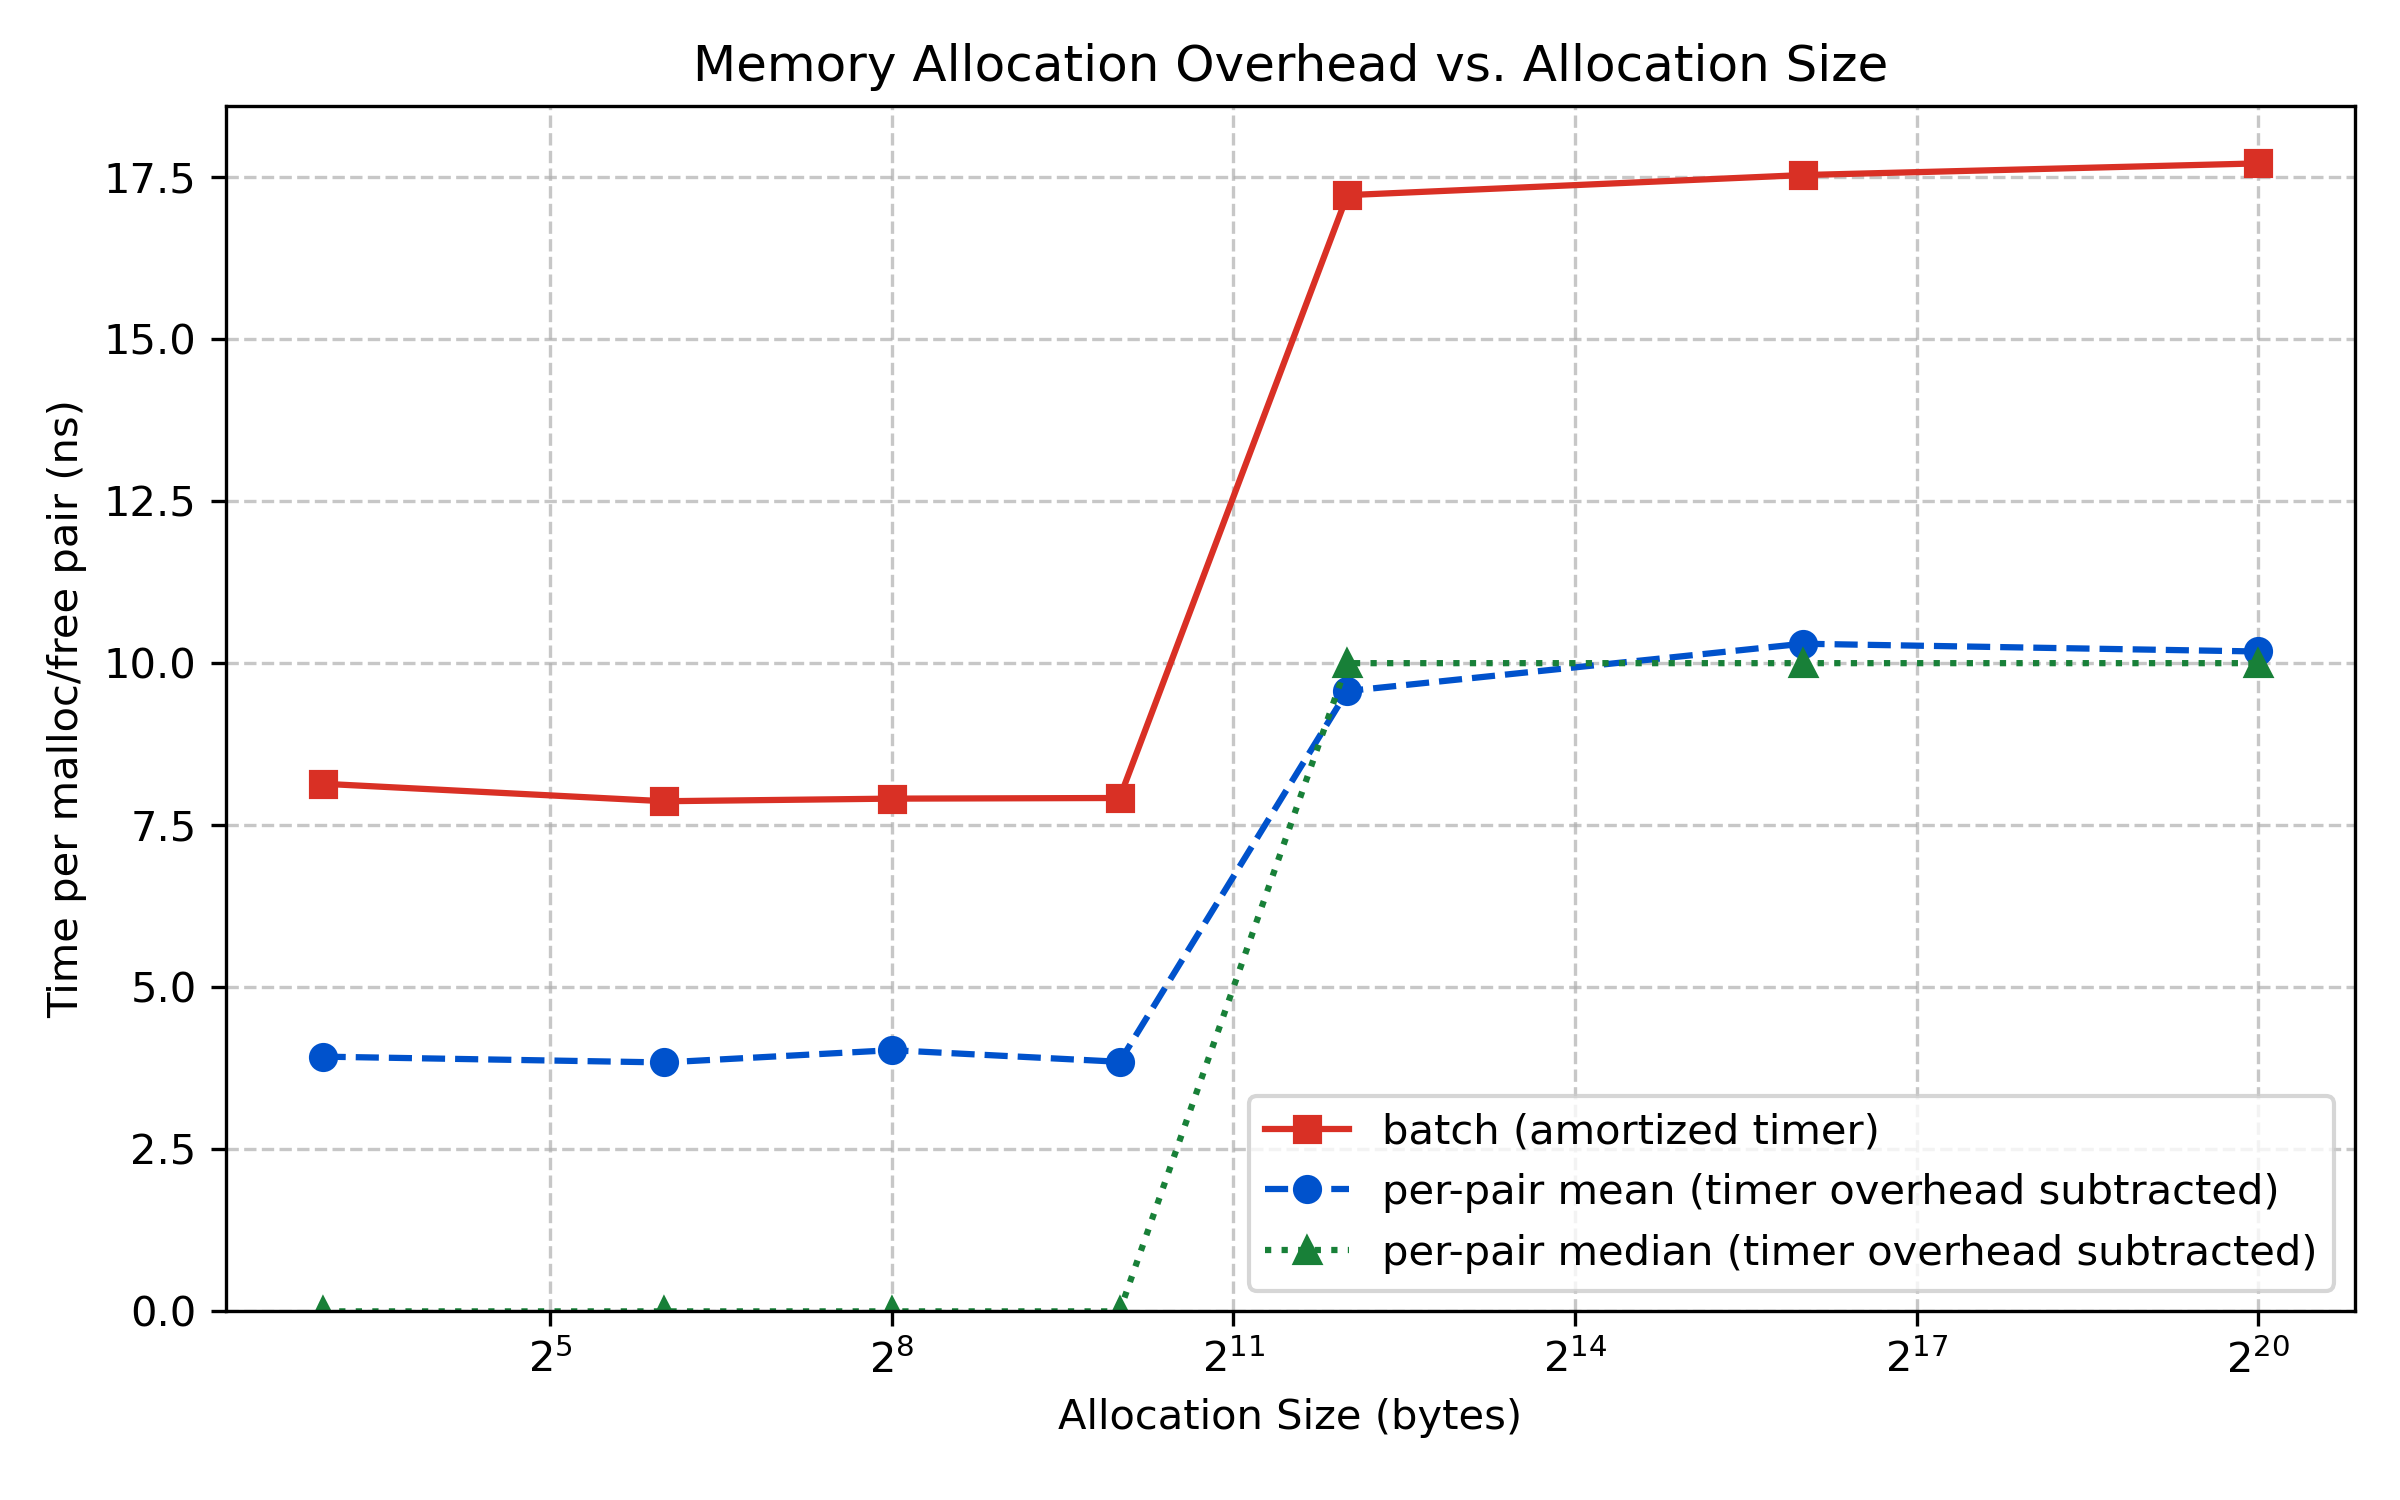
\includegraphics[width=0.75\textwidth]{figure_2_malloc_overhead.png}
    \caption{Time per malloc/free pair versus allocation size. Batch measurement takes the average of all iterations, and per-pair statistics have the timer overhead subtracted.}
    \label{fig:malloc_overhead}
\end{figure}

In figure \ref{fig:malloc_overhead} we see that there are two levels of latency for
the malloc/free pairs. The lower one ($\approx8ns$) exists likely because of the thread cache, and
the higher level ($\approx17ns$) exists because the thread cache is exceeded, but the warmup already
raised the threshold for larger allocations, which makes this level also stay somewhat constant.

% ============================================================
\newpage
\section{Hardware Info}\label{section:hardware_info}
% ============================================================

\subsection{Jort Oosterveld}

Type of computer: Laptop \\
Operating system: Ubuntu 24.04.4 LTS \\
Kernel version: Linux 7.0.0-38-generic \\
Hardware Model: Acer Aspire AG15-42P \\
Graphics: AMD Radeon Graphics

\begin{lstlisting}[caption=From lshw]
description: Computer
width: 64 bits
capabilities: smp vsyscall32
*-core
     description: Motherboard
     physical id: 0
   *-memory
        description: System memory
        physical id: 0
        size: 15GiB
   *-cpu
        product: AMD Ryzen 7 5825U with Radeon Graphics
        vendor: Advanced Micro Devices [AMD]
        physical id: 1
        bus info: cpu@0
        version: 25.80.0
        size: 3629MHz
        capacity: 4547MHz
        width: 64 bits
\end{lstlisting}

\begin{lstlisting}[caption=From lscpu]
$ lscpu --cache

NAME ONE-SIZE ALL-SIZE WAYS TYPE        LEVEL SETS  PHY-LINE COHERENCY-SIZE
L1d       32K     256K    8 Data            1   64         1             64
L1i       32K     256K    8 Instruction     1   64         1             64
L2       512K       4M    8 Unified         2 1024         1             64
L3        16M      16M   16 Unified         3 16384        1             64
\end{lstlisting}

\subsection{Sergiu Preda}

Type of computer: Laptop \\
Operating system: Windows 11 with WSL Ubuntu 22.04 LTS \\
Kernel version: Linux 6.18.33.2-microsoft-standard-WSL2 \\
Hardware Model: ASUS ROG TUF F15 \\
Memory: 7.6GiB

\begin{lstlisting}[caption=From lscpu]
Model name:            12th Gen Intel(R) Core(TM) i7-12700H
Flags:                 ... avx2 ...
\end{lstlisting}

\begin{lstlisting}[caption=From lscpu --cache]
$ lscpu --cache
NAME ONE-SIZE ALL-SIZE WAYS TYPE        LEVEL  SETS PHY-LINE COHERENCY-SIZE
L1d       48K     480K   12 Data            1    64        1             64
L1i       32K     320K    8 Instruction     1    64        1             64
L2       1.3M    12.5M   10 Unified         2  2048        1             64
L3        24M      24M   12 Unified         3 32768        1             64
\end{lstlisting}

For additional microarchitecture information, the following sources
were used:

\begin{itemize}
    \item uops.info instruction latency and throughput database: \url{https://uops.info/}
    \item Agner Fog instruction tables: \url{https://www.agner.org/optimize/instruction_tables.pdf}
\end{itemize}


% -----------------------------------------------
% appendix
% -----------------------------------------------
\newpage
\appendix

\end{document}
